This section describes the datasets, targets, data splitting strategies, training protocols, and evaluation procedures used in all experiments.

\subsection{Datasets and Targets}

We evaluate all models on multiple datasets of organic chromophores and fluorophores with experimentally measured optical properties. Across all datasets, the prediction targets are peak absorption and/or emission wavelengths reported in nanometers (nm). Each dataset differs in size, chemical diversity, and application domain, enabling systematic evaluation across data regimes.

The largest dataset, Deep4Chem~\cite{joung2020experimental}, contains experimentally measured absorption and emission wavelengths for a chemically diverse collection of organic molecules compiled from the literature. To probe transfer learning and robustness under reduced data availability, we additionally consider smaller, domain-specific datasets, including the Dye-Sensitized Solar Cell Database (DSSCDB)~\cite{venkatraman2018dye}, the ChemFluor dataset~\cite{ju2021machine}, and the Jeffries-EL dataset~\cite{tannir2024predicting} of blue-emitting benzobisoxazole-based OLEDs. The Jeffries-EL dataset is substantially smaller and is primarily used as a qualitative case study rather than for full model benchmarking.

To provide a qualitative overview of the chemical diversity and overlap across datasets, we visualize the global organization of molecular space using a two-dimensional Uniform Manifold Approximation and Projection (UMAP) embedding (Figure~\ref{fig:umap_pub_final}). Each point corresponds to a molecule, coloured by dataset.

\begin{figure}[ht]
  \centering
  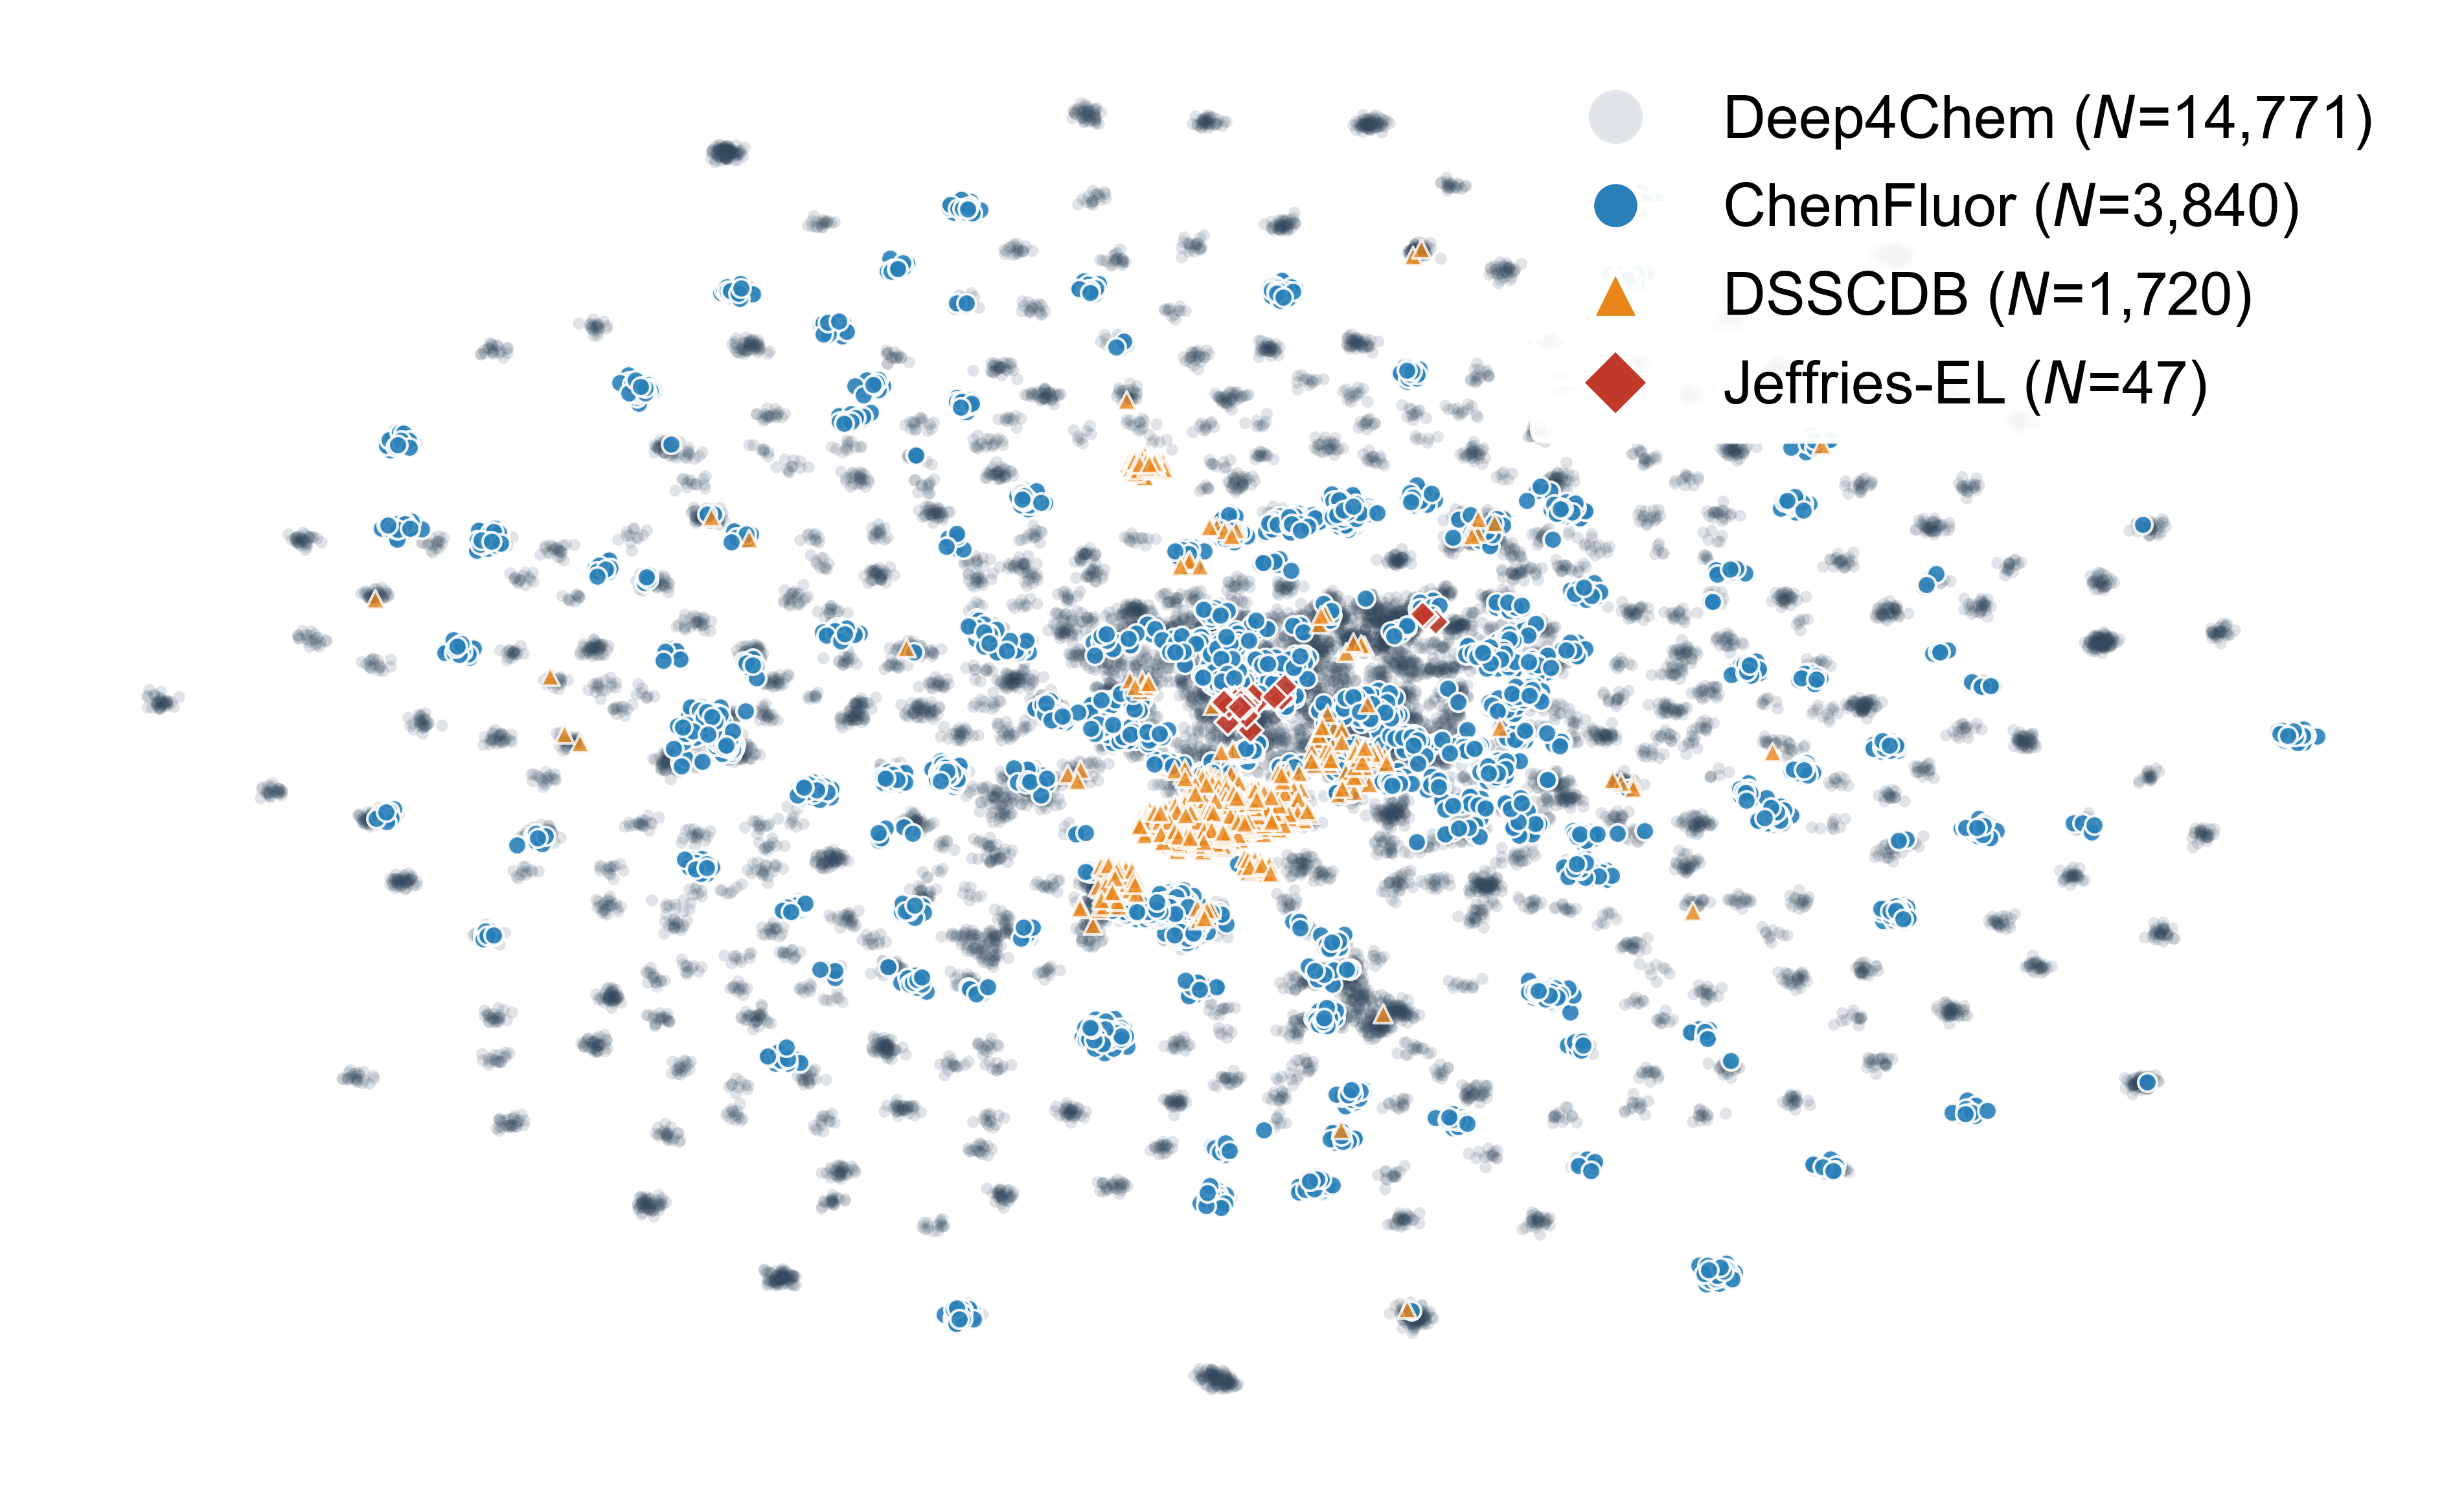
\includegraphics[width=0.9\linewidth]{figures/umap_pub_final.png}
  \caption{\textbf{Qualitative comparison of dataset chemical space.} Two-dimensional UMAP projection of molecules from all datasets computed from 2048-bit Morgan fingerprints (radius 2) using the Jaccard distance. To reduce overplotting due to repeated structures (e.g., identical fingerprints across solvents), points are displayed with a small random jitter.}
  \label{fig:umap_pub_final}
\end{figure}

All datasets were preprocessed following the protocol of Greenman \textit{et al.}~\cite{greenman2022multi} without modification. Molecular structures were canonicalized using RDKit, and only solution-phase measurements were retained; solid-state measurements were excluded. For molecules with multiple reported measurements in the same solvent, entries were filtered based on consistency: measurements differing by more than 5~nm were discarded, while remaining duplicate measurements were averaged. Measurements corresponding to the same molecular structure in different solvents were treated as distinct datapoints through solvent-specific feature representations. 

For datasets containing both absorption and emission measurements, the number of usable datapoints differs between targets due to incomplete experimental coverage. All analyses were therefore conducted on target-specific subsets derived from the same underlying molecular pool. Unless otherwise noted, dataset sizes $N$ refer to datapoints rather than unique molecules. A summary of dataset sizes and target availability is provided in Table~\ref{tab:datasets}.


\begin{table}[ht]
\centering
\caption{Summary of datasets used for optical property prediction after preprocessing.
Counts are reported as Absorption / Emission where applicable.}
\label{tab:datasets}
\begin{tabular}{l l c c}
\toprule
\textbf{Dataset} 
& \textbf{Target(s)} 
& \textbf{Datapoints} 
& \textbf{Unique Molecules} \\
\midrule
Deep4Chem 
& Abs., Emis. 
& 14{,}771 / 14{,}378 
& 5{,}841 / 5{,}597 \\

DSSCDB 
& Abs., Emis. 
& 1{,}720 / 690 
& 1{,}647 / 674 \\

ChemFluor 
& Abs., Emis. 
& 3{,}840 / 3{,}953 
& 2{,}622 / 2{,}617 \\

Jeffries-EL 
& Emis. 
& 47 
& 47 \\
\bottomrule
\end{tabular}
\end{table}

\subsection{Data Splitting and Training Regimes}

To assess generalization under both interpolation and distribution shift, we employ two splitting strategies. Random splits are used to approximate in-distribution generalization, while Bemis--Murcko scaffold splits are used to evaluate extrapolation to unseen chemical scaffolds. We adopt the same random and Bemis--Murcko scaffold splitting procedures as Greenman \textit{et al.}~\cite{greenman2022multi} and verify split equivalence by matching scaffold assignments and split indices.
To quantify the effective degree of distribution shift induced by each splitting strategy, we compute the maximum test-to-train Tanimoto similarity for all test molecules under both random and scaffold splits (Figure~\ref{fig:split-validation}). As expected, scaffold splitting substantially reduces train–test chemical overlap for Deep4Chem and ChemFluor, while DSSCDB exhibits comparatively high similarity even under scaffold splits, consistent with its narrower chemical diversity.

\begin{figure*}[t]
  \centering
  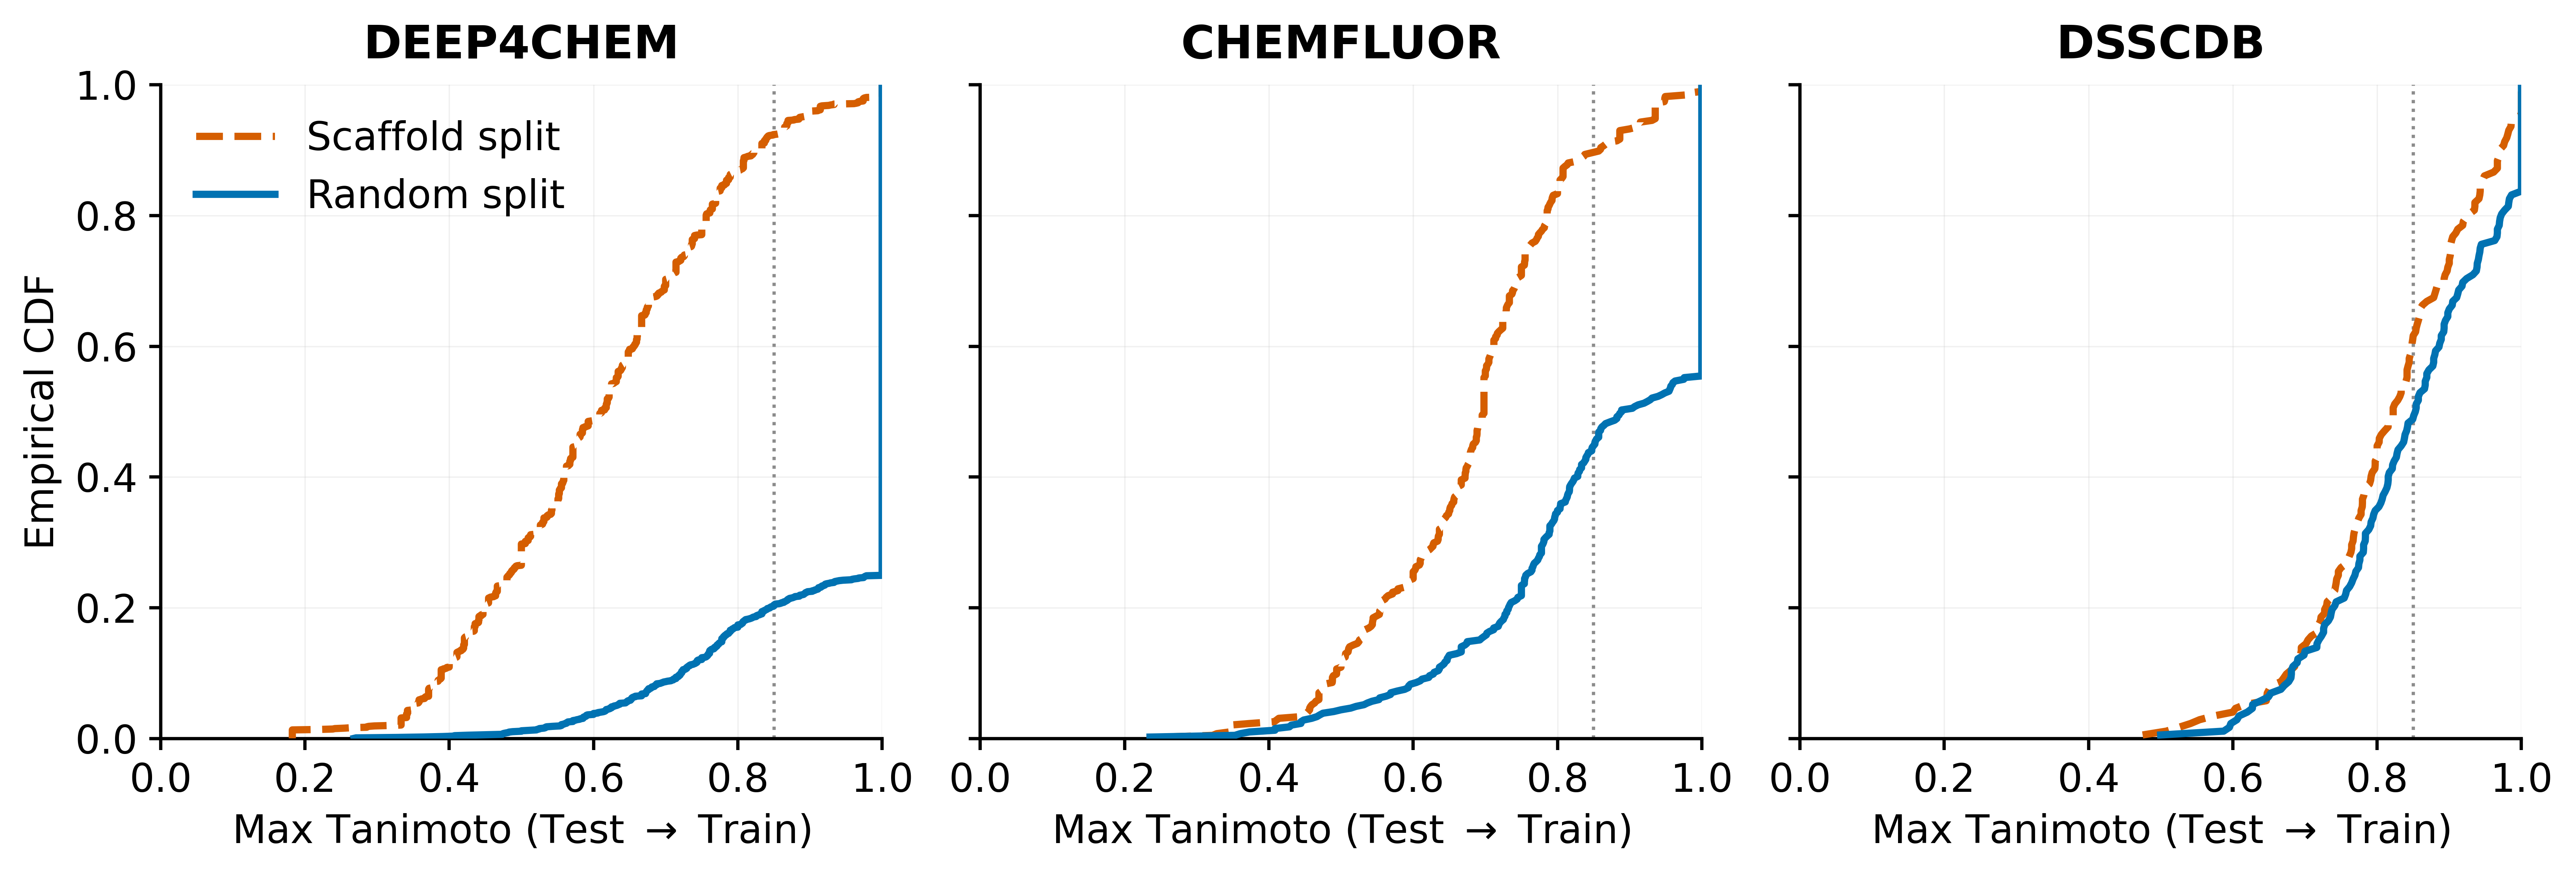
\includegraphics[width=0.9\linewidth]{figures/split_validation_cdf.png}
  \caption{\textbf{Train–test chemical similarity under random and scaffold splits.}
Empirical cumulative distribution functions (CDFs) of the maximum Tanimoto similarity between each test molecule and the training set, computed using Morgan fingerprints, for random and Bemis--Murcko scaffold splits across Deep4Chem, ChemFluor, and DSSCDB.
Vertical dotted lines indicate a commonly used similarity threshold ($T=0.85$), above which molecules are typically considered highly similar.
Scaffold splits substantially reduce train–test chemical overlap for Deep4Chem and ChemFluor, while DSSCDB exhibits higher intrinsic similarity across splits, reflecting its more chemically homogeneous composition.}

  \label{fig:split-validation}
\end{figure*}

\paragraph{Fixed subsampling for data-regime experiments.}
To evaluate performance as a function of training set size $N$, we constructed fixed subsampled training sets from each canonical split. For a given dataset, target, and split type, the original validation and test sets were held fixed, and training subsets were generated by sampling without replacement from the canonical training pool at sizes $N \in \{50,100,250,1000,4000\}$, as well as the full training set where available. For datasets with smaller training pools, only the feasible subset sizes were considered. Subsampling was performed using a fixed random seed, and the same subsampled training sets were reused across all model architectures and random initialization runs to ensure that differences across $N$ reflect model behaviour rather than variation in the sampled training examples. For hybrid models, downstream heads were trained on embeddings extracted from the corresponding subsampled training set, with validation and test evaluation performed on the fixed canonical splits. 


\subsection{Model Training Protocols}

\paragraph{End-to-end D-MPNN training.}
For each data regime, we conducted a 200-trial Optuna Bayesian hyperparameter search over architectural and optimization parameters, including network depth, FFN capacity, dropout rate, batch size, and learning-rate schedule. Optimization was performed using the Adam optimizer with a learning-rate warmup schedule and mean squared error (MSE) loss. We fixed the hidden dimension of the encoder at 482, consistent with Greenman \textit{et al.}~\cite{greenman2022multi} to ensure a consistent representational capacity across all data regimes and to mitigate numerical instability observed in ultra-small $N$ settings when the hidden dimension was allowed to vary.

Unless explicitly tuned, all remaining parameters were set to Chemprop defaults. Models were trained for a fixed 200 epochs without early stopping. This protocol was chosen to strictly isolate the impact of dataset size on training dynamics, avoiding the confounding influence of varying stopping criteria across data regimes. For each data regime, the optimal hyperparameter configuration identified by Optuna was reused across all ensemble members. To verify that fixed training horizons do not induce late-stage overfitting, we inspected training and validation trajectories across representative small- and large-data regimes and observed stable convergence without divergence in validation error (see Figure~\ref{fig:si-convergence}).

\paragraph{Hybrid model training.}
For the hybrid paradigm, D-MPNN encoders were pretrained as described above, then frozen. The downstream XGBoost heads were tuned via a separate 100-trial Optuna search for each $N$, optimizing tree depth, learning rate ($\eta$), and regularization terms ($\lambda, \alpha$).

\paragraph{Ensembling and Reproducibility.}
To mitigate stochasticity arising from random initialization and training dynamics, all reported performance metrics are based on ensemble predictions unless otherwise noted.
\begin{itemize}
\item \textbf{Deep and Hybrid Models:} Ensembles consist of $M=5$ independently trained models (distinct random seeds) sharing the same hyperparameter configuration. For hybrid models, this involves pairing 5 independently trained encoders with 5 corresponding downstream heads.
\item \textbf{Gradient-Boosted Baselines:} Due to their low computational cost, tree-based baselines are evaluated using larger ensembles of $M = 30$ models. 
\end{itemize}

\subsection{Evaluation Metrics}

Model performance is evaluated using Root Mean Squared Error (RMSE) computed on the held-out test set. All reported results correspond to the RMSE of the ensemble-averaged prediction. Where shown, error bars denote 95\% percentile bootstrap confidence intervals for the test RMSE, computed by resampling test molecules with replacement (2000 replicates). These intervals reflect sampling variability of the evaluation set and do not quantify variability across random initializations or ensemble members.


All deep learning models were implemented using PyTorch (v1.12) within the Chemprop framework (v1.6.1)~\cite{yang2019analyzing}. Chemical informatics operations and featurization were performed using RDKit (v2022.03.1), and gradient-boosted tree models were implemented using XGBoost (v1.6.2). Training and evaluation were conducted on NVIDIA H100 GPUs.

To ensure reproducibility, all code, canonical data splits, and trained model checkpoints used in this thesis are available at \url{https://github.com/michaelmontemurri/uvvis-hybrid-gnn}.
